
\documentclass[book.tex]{subfiles}
\begin{document}
In 1990 a small company based in Shreveport, Louisiana was doing well on the shareware market. As a video game subscription service, Softdisk produced and mailed new games every month to its members. Business was good but some of its employees had other ambitions. They thought they had the skills to make it big and they wanted to prove it.\\
\par
They had created a new way to program side scrolling. They called the technology "Adaptive tile refresh" and it enabled hardware scrolling on a PC capable of rivaling with a NES. In early 1990 they worked non stop during a weekend to reimplement Super Mario 3 on a PC and demonstrate their skills to Nintendo. They were successful in building a clone of Mario but unfortunately, "Ideas from the Deep" as they called themselves failed to convince the company to give them a contract. As impressed as they were, the Japanese firm wanted the Mario series to remain exclusive to Nintendo consoles.\\
\par
\begin{fancyquotes}
We sent this demo to Nintendo of America, they in turn sent it to Kyoto to the mothership office, and the execs there saw the demo and were really impressed. However, they didn't want their intellectual property on anything but their own hardware, so they told us Good Job and You Can't Do This.\footnote{Super Mario Bros. 3 Demo (1990) by John Romero: https://vimeo.com/148909578}
 \bigskip \\
\textbf{John Romero - Programmer}
 \end{fancyquotes}

 \begin{figure}[H]
   \fullimage{mario_ifd.png}
\caption{Mario 3 on PC. Notice the "IFD" for "Ideas From the Deep".}
\end{figure}

\par
This episode was enough to convince them they had not only the talent to feed their ambitions, but also the teamwork and work ethic to potentially go all the way. In February 1991 four Softdisk employees took the leap of faith and founded their own company. They named it "id Software"\footnote{For ample details, read "Masters of Doom" by David Kushner.}. 

 \begin{figure}[H]
\centering  
\begin{tabularx}{\textwidth}{ X  X  X  }
  \toprule
  \textbf{Name} &  \textbf{Age} & \textbf{Occupation} \\
  \toprule 
   John Carmack & 22 &  Programming\\
   John Romero & 25 &  Programming\\
   Adrian Carmack & 22 &  Artist\\
   Tom Hall & 28 &  Creative Director\\
     \toprule
\end{tabularx}
\caption{id Software founding members.}\label{fig:Id Software team}
\end{figure}
They immediately used the technology developed for "Mario 3 PC" to release their own titles and build their own intellectual property. Wasting no time, the team shipped no less than three titles in a year.
\begin{itemize}
    \item Commander Keen Episode 1,2 and 3: Invasion of the Vorticons (December 14th, 1990)
    \item Commander Keen Episode 4, 5 and 6: Good Bye Galaxy (December 15th, 1991)
    \item Commander Keen Standalone game: Aliens Ate My Baby Sitter (December 1991)
\end{itemize}
The games, published by FormGen, were instant successes and sold very well. They also kept on writing games for Softdisk to publish, most using Adaptive tile refresh.
\begin{itemize}
  \item Commander Keen in Keen Dreams (1991)
  \item Dangerous Dave in the Haunted Mansion (1991)
  \item Rescue Rover (1991)
  \item Rescue Rover 2 (1991)
  \item Shadow Knights (1991)
  \item Hovertank 3D (April, 1991).
  \item Catacomb 3D: A New Dimension (November, 1991)
\end{itemize}
During Spring 1991 the next generation of id Software technology started to surface\footnote{You can see screenshots in the Annex section.}. Hovertank 3D allowed the player to be inside a tank. There was no texture mapping yet and the pace was quite slow. Catacomb 3D marked the introduction of textures and took immersion one step further by placing the player in control of a magician in first person view. \\
\par

In November 1991, the team was free from any obligations to SoftDisk. The next game was going to use the 3D technology they were building and it would be called Wolfenstein 3D. Considering the magnitude and ambition of the title, four more people were added to the team for a total of eight.\\
\note{TODO Ask team members if they know how old were Jay, Bobby, Robert and Jason}
 \begin{figure}[H]
\centering  
\begin{tabularx}{\textwidth}{ X  X  X  }
  \toprule
  \textbf{Name} &  \textbf{Age} & \textbf{Occupation} \\
  \toprule 
   Jay Wilbur & ?? &  Business\\
   Kevin Cloud\protect\footnotemark{} & 27 &  Computer Artist\\
   Robert Prince & ?? &  Composer\\
   Jason Blochowiak\protect\footnotemark{} & ?? &   Programming\\
     \toprule
\end{tabularx}
\caption{id Software hires.}\label{fig:Id Software hires}
\end{figure}

\begin{fancyquotes}
Jason was part of id at the start, but we parted ways during Wolf development.
 \bigskip \\
\textbf{John Carmack - Programmer}
 \end{fancyquotes}
 \footnotetext{Jay and Kevin were recruited on April 1st, 1992 but were still given credits for participating to the game development.}
 \footnotetext{Jason wrote part of the page manager and is credited for introducing John Carmack to Unix development,
which ultimately led to the purchase of a Next ColorStation.}
 
\begin{figure}[H]
\centering
  \shadowbox{
      \fullimage{idTeam_team_pants.png}
  }  
\caption{The team as it appears in Spear of Destiny, in a secret screen created by John Romero.}
\label{fig:id_team_1993}
\end{figure}
 
\begin{figure}[H]
\centering
  \shadowbox{
      \fullimage{id_team_with_pants.jpg}
  }  
\caption{They were in fact wearing pants.}
\label{fig:id_team_1993}
\end{figure}


Development took seven months (from November 1991 to May 1992) during which id Software was located in Madison, WI. They relocated in August 1991 from Shreveport following Tom and Jason's rose-tinted school memories of the area.
\begin{figure}[H]
\centering
 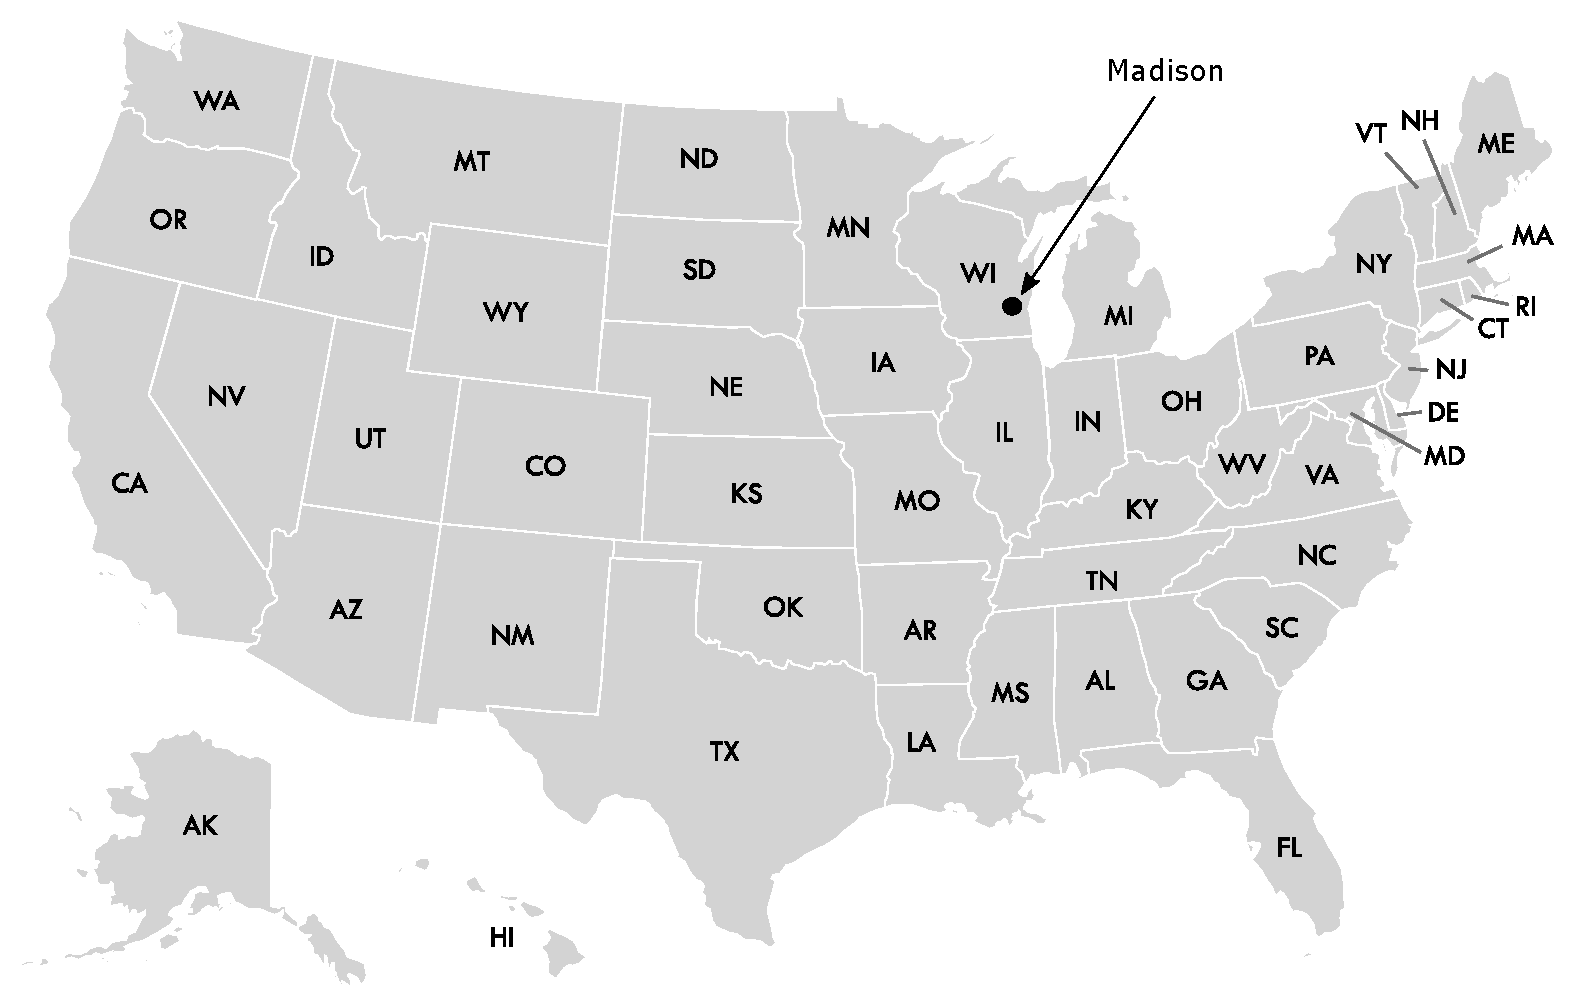
\includegraphics[width=\textwidth]{imgs/drawings/map/usa-id-software.eps}
 \end{figure}








\section{Organization}
The organization of the team was pretty much standard for a game studio of this era. Four guys crammed in one room which dictated a fast pace and strong sense of camaraderie (and a lot of noise disturbance given John Romero and Tom Hall's type of interaction). On the map (next page) you can see on the upper floor the SNES where countless games of F-Zero were played and the Dungeons \& Dragons area extensively mentioned in "Masters of Doom". To have a team member (John Carmack) with his apartment directly above the studio was not out of the ordinary\footnote{ "90 Hours A Week And Loving It!" by Andy Hertzfeld.}. The team's space was setup as follows.
\par
\begin{figure}[H]
  \centering
  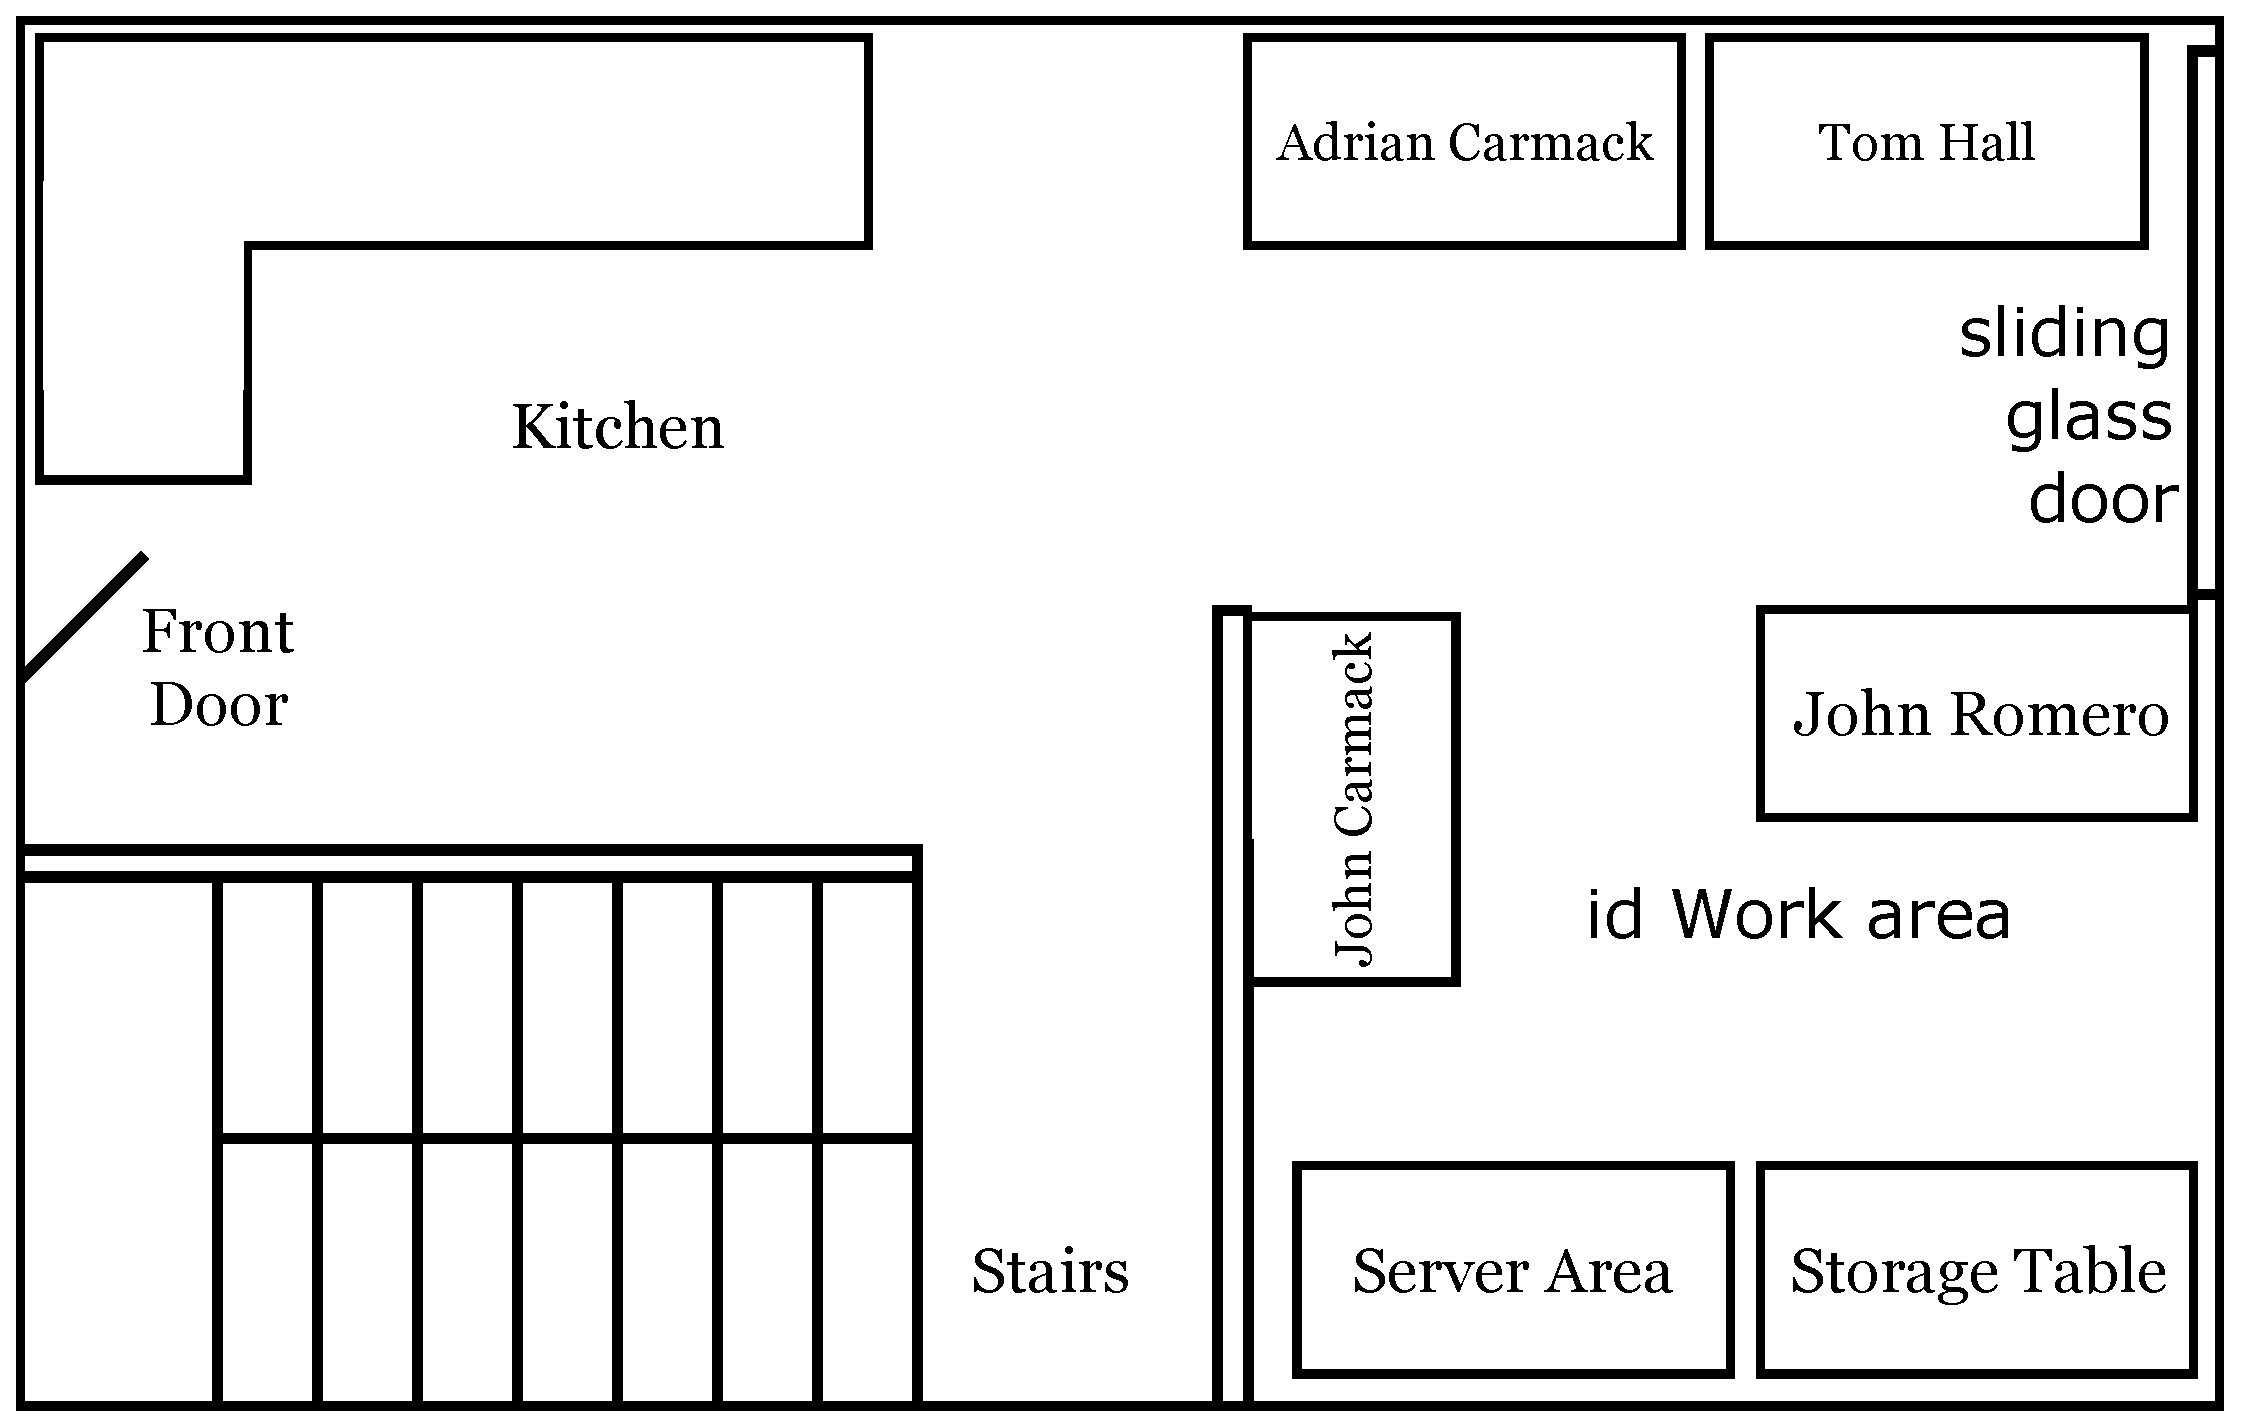
\includegraphics[width=\textwidth]{imgs/drawings/map/id-software-office-madison_bottom_floor.eps}
 %\caption{Office bottom floor.} 
\end{figure}
\par
\begin{figure}[H]
  \centering
  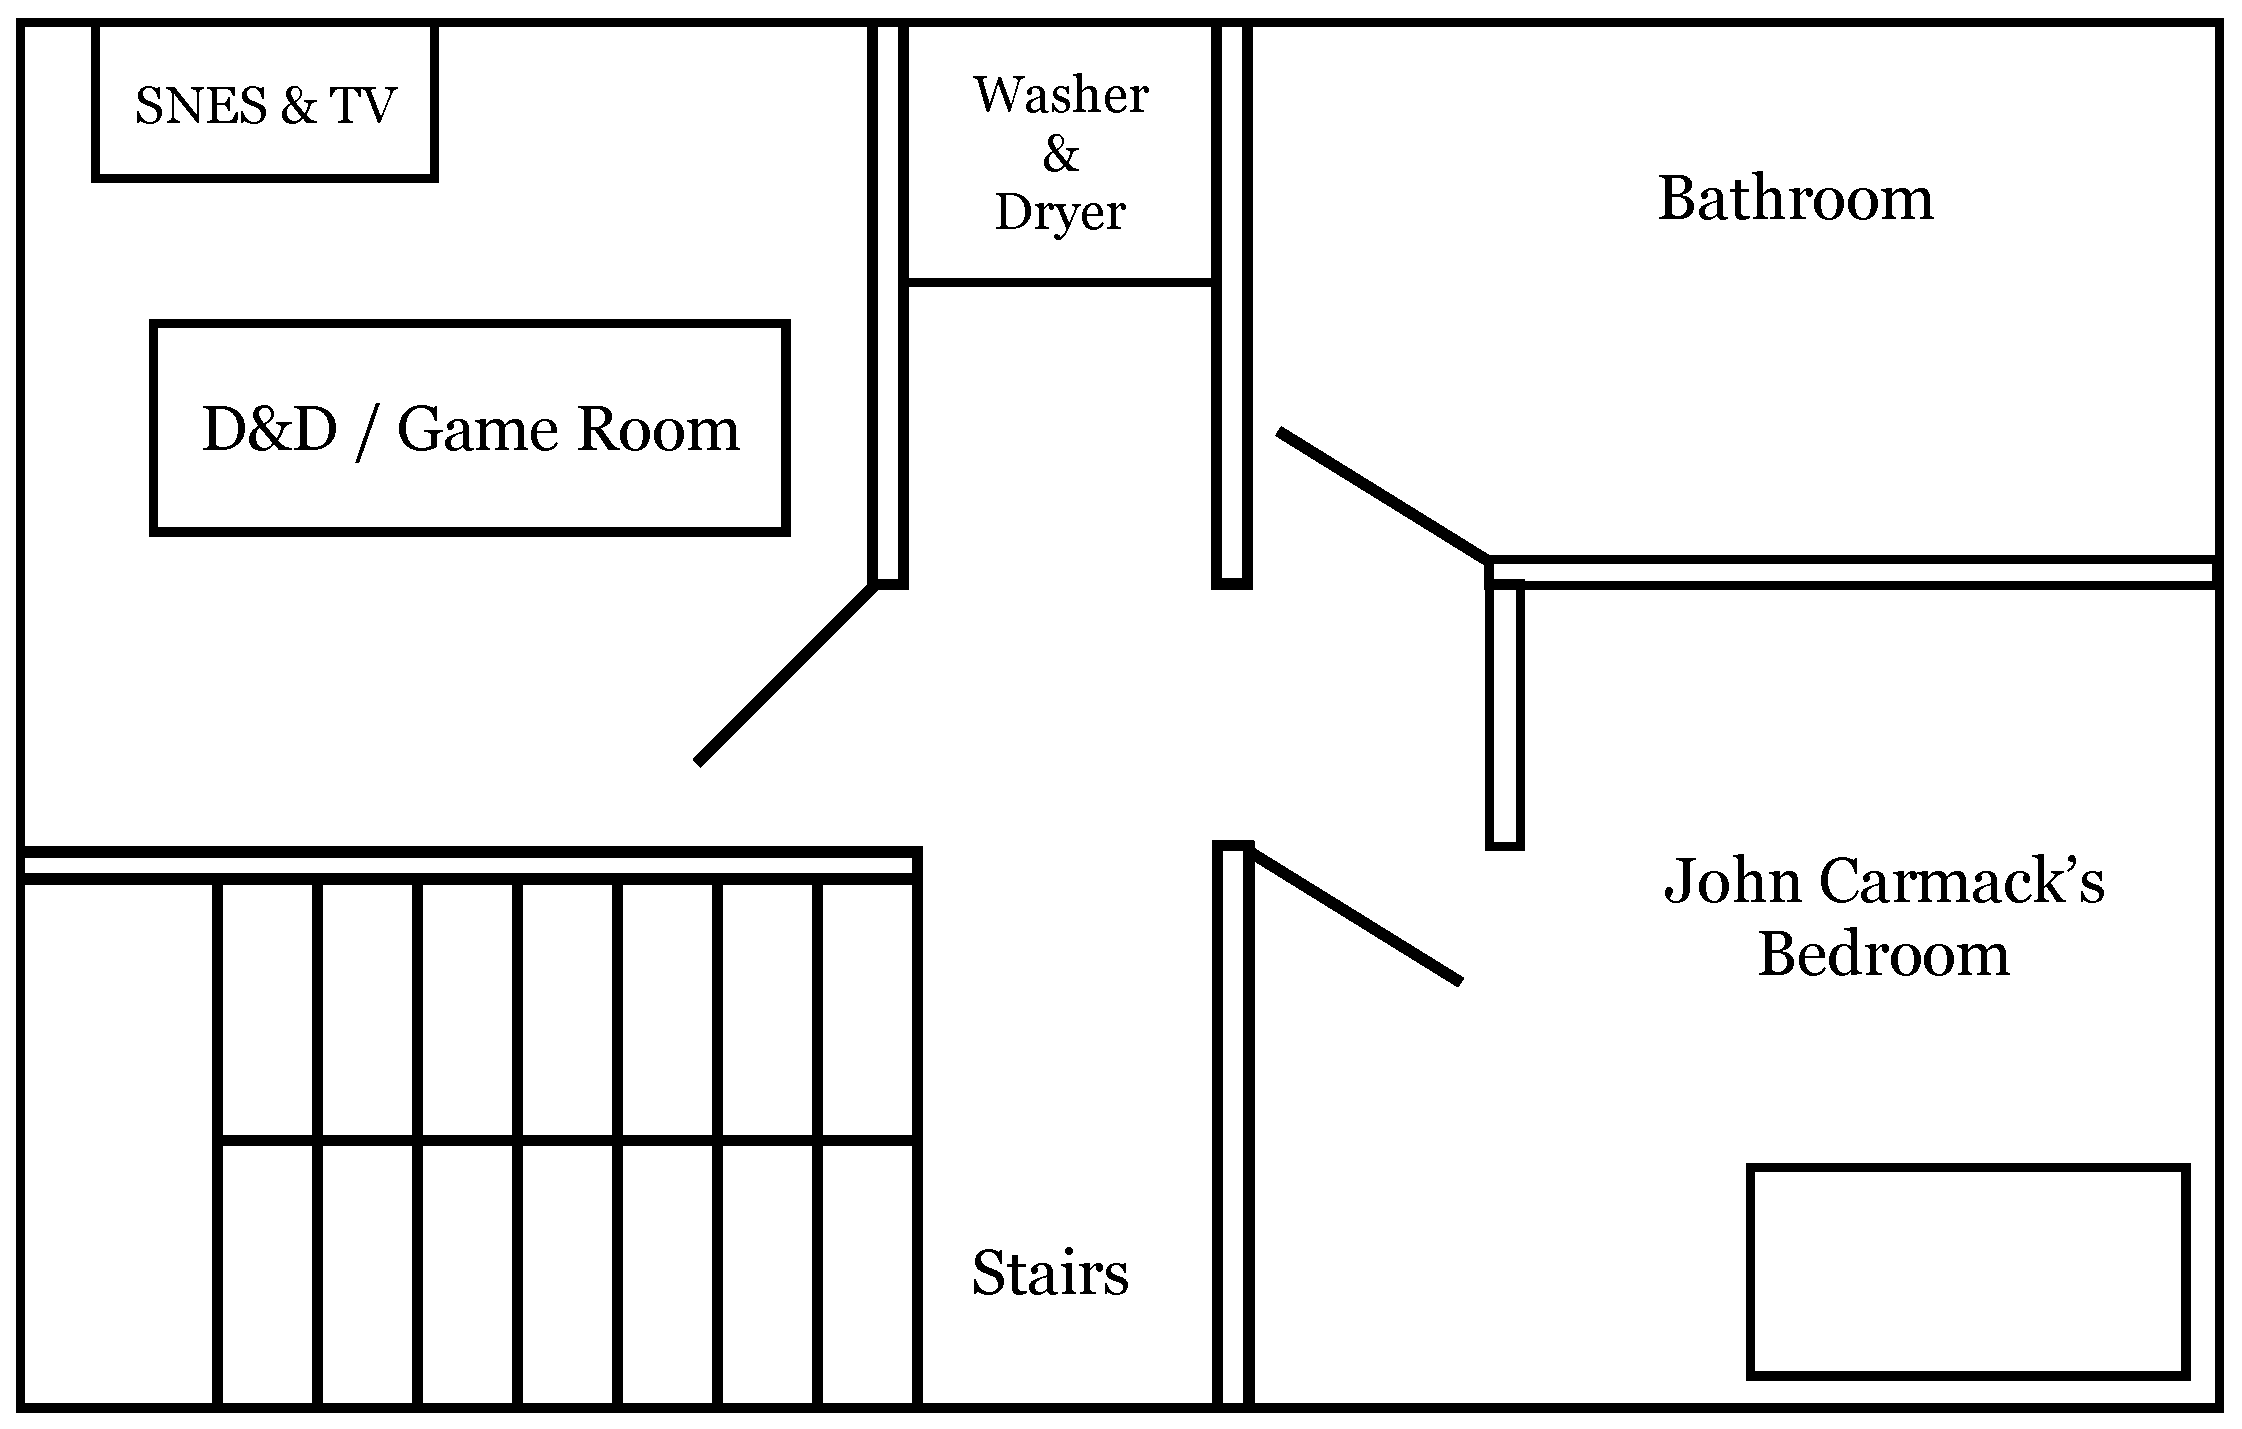
\includegraphics[width=\textwidth]{imgs/drawings/map/id-software-office-madison_top_floor.eps}
 %\caption{Office top floor.} 
\end{figure}
Everybody was working with the best PC money could buy, a high end 386-DX 33Mhz with 4MiB of RAM. As for combining engine, tools, and assets:\\

 \begin{fancyquotes}
We started with floppy data transfer, but we had a Novell network on coax Ethernet by the end. We didn't have a version control system.  Surprisingly, we went all the way to Quake 3 without one, then we started using Visual Source Safe.\\
 \\
\textbf{John Carmack - Programmer}
\end{fancyquotes}


























\section{Programming}



Development was done with Borland C++ 3.1 (but the language used was C). The editor uses VGA mode 3 offering a screen 80 characters wide and 25 characters tall.\\
\par
John Carmack took care of the runtime code. John Romero programmed many of the tools (TED map editor, Graphic assets packers, Muse sound packer). Jason Blochowiak was contracted to write important subsystems of the game (Input manager, Page Manager, Sound Manager, User Manager).\\
\\
\begin{figure}[H]
\centering
  \shadowbox{\fullimage{development.png}}  
\caption{Borland C++ 3.1 editor}
\end{figure}


To compensate for the tiny CRT display, some of the developers used two screens (an unusual thing at the time).\\

\begin{fancyquotes}
At that point, we wanted 21" monitors, but couldn't justify them.  I used a second mono monitor to allow Turbo Debugger 386 to keep the main screen in graphics mode while I stepped through the code.\\
 \\
\textbf{John Carmack - Programmer}
\end{fancyquotes}
\\
You may have noticed in the listing of VGA modes that \cw{Mode 13h} and \cw{Mode 4h} (figure~\ref{fig:vga_modes} on page~\pageref{fig:vga_modes})  don't have the same starting RAM address. This allows a trick where two graphic cards are plugged in the same PC. One MDA setup as monochrome text mode picks up data at 0xB8000 while a VGA mapped at 0xA0000 runs the game normally. This setup allows a developer to debug the game engine with breakpoints.\\
\begin{figure}[H]
\centering
  \shadowbox{
      \fullimage{wolf_screen1.png}
  }  
\caption{Monitor 1 with Borland Turbo Debugger 386}
\label{fig:dm1}
\end{figure}

\begin{figure}[H]
\centering
  \shadowbox{
      \fullimage{wolf_screen2.png}
  }  
\caption{Monitor 2 running the game as normal}
\label{fig:dm1}
\end{figure}



 
 
 




\section{Graphics assets}

All graphic assets were produced by Adrian Carmack\footnote{Kevin Cloud did a few textures and also worked on the design and layout of the Wolfenstein 3D hint book published eventually.}. All of the work was done with Deluxe Paint (from Electronic Arts) and saved in LBM files (Deluxe Paint format). 

\begin{figure}[H]
  \centering
 \fullimage{deluxe_paint.png}
 \caption{Deluxe Paint was used to draw all assets in the game.}
\end{figure}


\par
Since the VGA is palette based (colors were not specified via 24-bit RGB but via indices pointing to a 256 colors table) the creative process was difficult. The artist had first to make the key decision of which colors would go in the palette\footnote{Some games like "Monkey Island" used many palettes depending on the section of the game. id Software went for a simpler solution with one palette for the whole game.} and then draw everything with only these colors.\\
\begin{figure}[H]
  \centering
\fullimage{palette.png}
 \caption{Wolfentein 3D palette: Everything in the game is drawn using these 256 colors.}
\end{figure}
The palette coordinates are horizontally from \cw{0x00} to \cw{0x0F} and vertically from \cw{0x00} to \cw{0xF0}. The horizontal blue gradient at the bottom starts at 0xF0 and ends at 0xFE. 0xFF (represented in pink) is a special color deemed transparent by the engine and always skipped during rendition.\\
\par

All assets were hand drawn with a mouse. Since the VGA stretched the framebuffer when displaying it on the screen (from 320x200 to 320x240), Adrian had to be careful to draw at the same resolution as the game would run.\\
\par
\begin{fancyquotes}
We didn't have any scanning tools at the time.\\
\\
\textbf{John Carmack - Programmer}
\end{fancyquotes}
\\
The graphic assets are divided in two categories:
\begin{itemize}
\item 2D Menu items shipping with the game in \cw{VGAXXXX} archive
\item 3D Action phase items (walls and sprites) shipping in the \cw{VSWAP} archive
\end{itemize}















\section{Assets workflow}
After the graphic assets were generated, a tool (IGRAB-ED) packed all the ILBMs files together in an archive and generated a C header file with asset IDs. The engine references an asset directly by using these IDs.\\
\begin{figure}[H]
\centering
 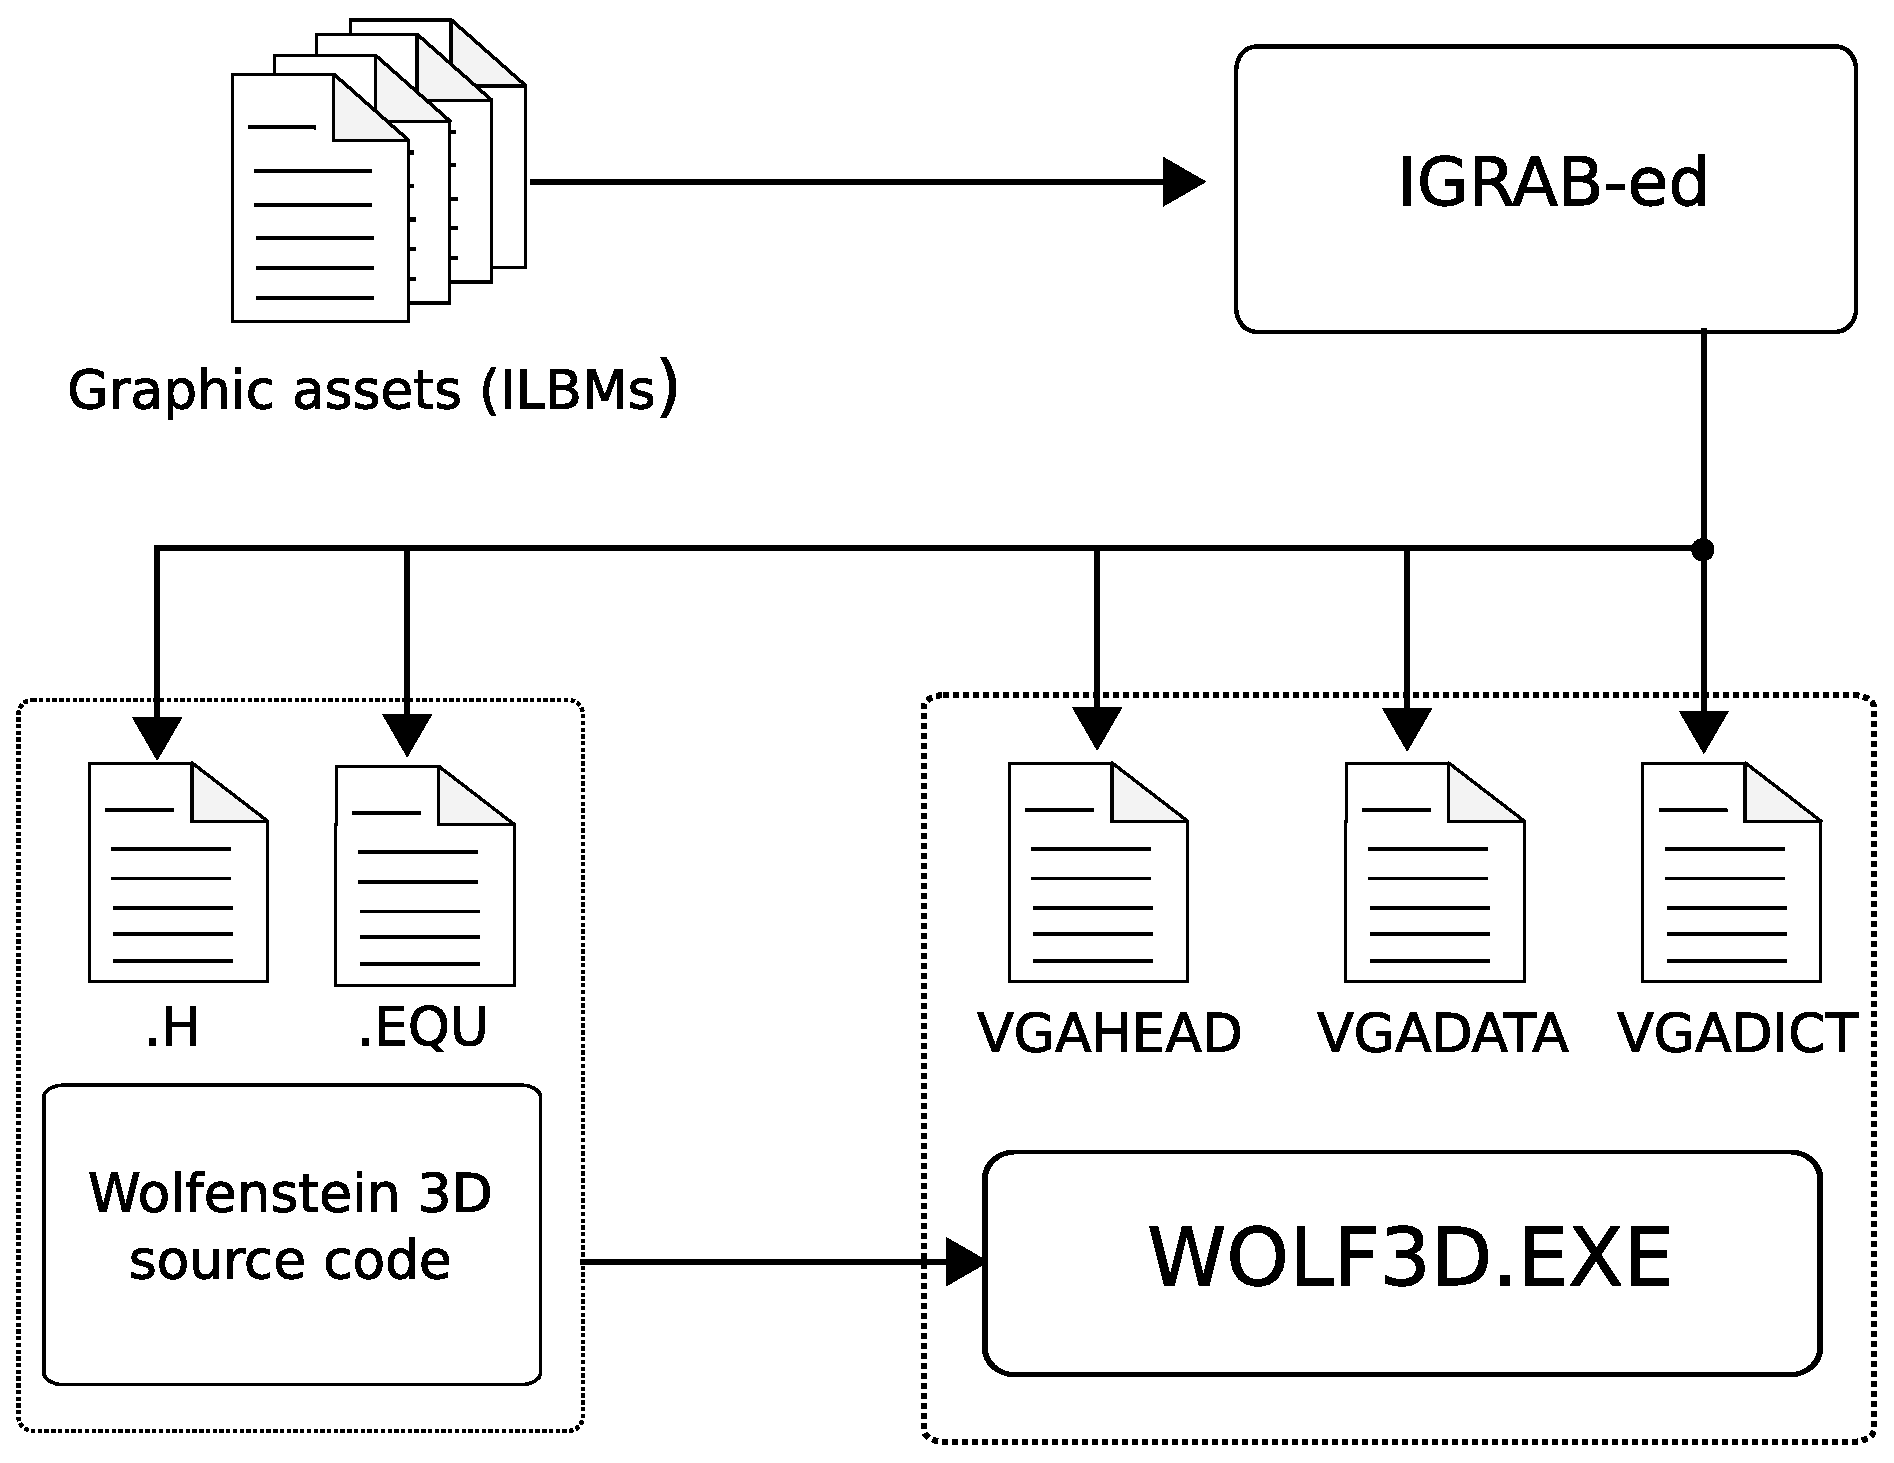
\includegraphics[width=\textwidth]{imgs/drawings/drawing_plain.eps}
 \caption{Asset creation pipeline for the 2D Menu items}
\end{figure}
\par
\begin{minipage}{\textwidth}
 \lstinputlisting[language=C]{code/assets_header.c}\par
 \end{minipage}
 
 In the engine code, asset usage is "hardcoded" via an enum. This enum is an offset into the 
 \cw{HEAD} dictionary which gives an offset in the \cw{DATA} archive. Thanks to this indirection layer, the assets could be regenerated and reordered at will with no modification in the source code.\\
 \par
 \begin{minipage}{\textwidth}
 \lstinputlisting[language=C]{code/assets_usage.c}\par
 \end{minipage}
\par
\textbf{\underline{Trivia :}} This system led to issues when the source code was released. The \cw{.h} header files provided did not match the assets files from the shareware or early version of Wolfenstein 3D. The headers released were from Spears of Destiny. You can see the kind of graphic mess this let to in the article "Let's compile like it is 1994" on \cw{fabiensanglard.net}.\\




\begin{minipage}{0.7\textwidth}
"The Official Hint Manual for Wolfenstein 3D" published in 1992 contains many drawings from Tom Hall and shows many behind the scene sketches made by Tom Hall and pixelarted by the graphic team.\\
\par
 \begin{fancyquotes}
When Id's Creative Director, Tom Hall gets an idea for a screen, he provides a sketches for Adrian Carmack. Below are some of Tom's early design for the title screen. The third sketch was chosen.\\
\end{fancyquotes}
\end{minipage}
\begin{minipage}{0.3\textwidth}
\begin{flushright}
\scaledimage{0.9}{hint_manual_cover.png}
\end{flushright}
\end{minipage}

\noindent
   \begin{figure}[H]
\centering
 \fullimage{sprites/tom_hall_sketch_intro_screen_genesis.png}
 \end{figure}
 \par
   \begin{figure}[H]
\centering
 \scaledimage{.7}{sprites/woldf3d.png}
\end{figure} 

\footnotetext{The manual was entirely designed on a NeXT ColorStation. It was the only usage of NeXT for Wolfenstein 3D (they purchased it in December 1991).}



\begin{figure}[H]
\centering    
     \fullimage{sprites/tom_hall_sketch_adolf.png}
   \end{figure}



     \begin{figure}[H]
\centering
     \fullimage{sprites/tom_hall_sketch_dr_schabbs.png}
   \end{figure}
 
  \begin{figure}[H]
\centering
 \scaledimage{0.8}{sprites/tom_hall_sketch_gretel.png}\\
 \end{figure}



     \begin{figure}[H]
\centering
     \scaledimage{0.9}{sprites/tom_hall_sketch_giftmacher.png}
   \end{figure}

     \begin{figure}[H]
\centering
     \scaledimage{0.9}{sprites/tom_hall_sketch_fettgesic.png}
   \end{figure}


\par 
The hint manual also contains several photos of the team back in the days; it is worth a read for context.













\section{Maps}
Maps were created using an in-house editor called TED5, short for Tile EDitor. TED was not created specially for Wolf 3D, but was originally made for the Commander Keen series and improved over the years. It was a versatile tool since it allowed for creating maps of side scroller games but also top-down games like Rescue Rover and Wolf 3D. TED5 does not stand-alone; in order to start, it needs an asset archive and the header associated (as described in the graphic asset workflow). This way, texture ids are directly encoded in the map.\\

 \begin{figure}[H]
\centering
 \fullimage{TedSplashscreen.png}
 \end{figure}

  \begin{figure}[H]
\centering
 \fullimage{Fill_2.png}
 \end{figure}


 \begin{figure}[H]
\centering
 \fullimage{ted5_scrolling_map.png}
 \caption{TED used for Commander Keen - side scroller} 
 \end{figure}

TED allows placement of tiles on layers called "planes". This layered approach proved powerful and versatile. In Commander Keep, layers are used for background tiles, which the hero can stand on, generating bonuses and so on. For Wolfenstein 3D two layers are used: one for walls, and another to place bonuses and enemies.\\
\begin{figure}[H]
\centering
 \fullimage{TED.png}
 \caption{TED used for top view level design in Rescue Rover.} 
 \end{figure}

Reusing TED5 was a double win. Not only did it save tool development time, but all team members had also been using it for years and were proficient, reducing ramp-up time. TED5 was so good at doing the job that it allowed designers to make a level within minutes.\\
\par

 \begin{fancyquotes}
After talking with Romero and Tom, Scott learned that it was taking the group only about one day to make a level of the game. Ka-chung! Dollar signs! Instead of just three episodes, why not have six? Scott said, "If you can do thirty more levels, it would only take you fifteen days. And we could have it where people could buy the first trilogy for thirty-five dollars or get all six for fifty dollars, or if people buy the first episode and later want the second episodes it will be twenty dollars. So there's a reason to get them all!" After some consideration, id agreed.\\
\\
 \textbf{- Masters of Doom}
 \end{fancyquotes}\\

\par
Everybody worked a little bit on the map but it was mostly the work of John Romero and Tom Hall.\\
\par
 \textbf{\underline{Trivia :}} The source code of TED5 was released several years later. Among the source code made of \cw{.C} and \cw{.H} was a mysterious \codeword{\_TOM.PIC}. It turned out to be a caricature of Tom Halls made by Adrian Carmac. The explanation was provided later by John Romero in 2002:\\
\par
 \begin{fancyquotes}
   "Hahahaha! Wow, I forgot all about that picture. I can't believe it's 
in the TED5 source files! It's basically a pic that Adrian drew of Tom 
[...] saying "Sorry!".\\
\par 
It's because Tom and Adrian used to share a worktable together and Tom 
would always bump the table while Adrian was drawing graphics with the 
mouse and Tom would say, "Sorry!" That picture never appears in Ted5 
anywhere.\\
   \\
\textbf{John Romero - Programmer}
 \end{fancyquotes}\\











\section{Audio}

\subsection{Sounds}
As mentioned in the hardware section, audio hardware was highly fragmented. id decided to support all four sound cards and the default PC speaker, which meant generating assets multiple times for each and packing them together with an in-house tool called MUSE into an AUDIOT archive (an id software proprietary format):\\
\begin{figure}[H]
\centering
 \fullimage{muse.png}
 \end{figure}
 \par
 Three sets of the same audio effect shipped with the game:
\begin{enumerate}
\item For PC Speaker
\item For Adlib
\item For SoundBlaster, SoundBlaster Pro and Disney Sound Source
\end{enumerate}

\par
All voices were recorded by John Romero and Tom Halls, faking german accents the best they could\footnote{Source:Masters of doom by David Kushner}.






\subsection{Music}
All music composition work was performed by Robert Prince.\\
\par
 \begin{fancyquotes}
In the early days of the OPL soundcards, the "gold standard" sequencing software was Sequencer Plus Gold ("SPG") by Voyetra. The reason for this was it had an OPL instrument/instrument bank editor.\\
\par
To rough out compositions, I used Cakewalk ("CW"). I had been using it for several years already and had it all set up to use the analog boxes for sound output. Having "real" sounds from those boxes helped me visualize (audiolize?) what I wanted musically. I would save the CW files in *.mid format and load them into SPG to create the OPL instrument for each track. I built different instrument banks for the different genres of music.\\
   \\
\textbf{Bobby Prince - Composer}
 \end{fancyquotes}\\

\begin{figure}[H]
\centering
  \shadowbox{
      \fullimage{music_editor.png}
  }  
\caption{Sequencer Plus Gold ("SPG") by Voyetra.}
\end{figure}

\begin{figure}[H]
\centering

 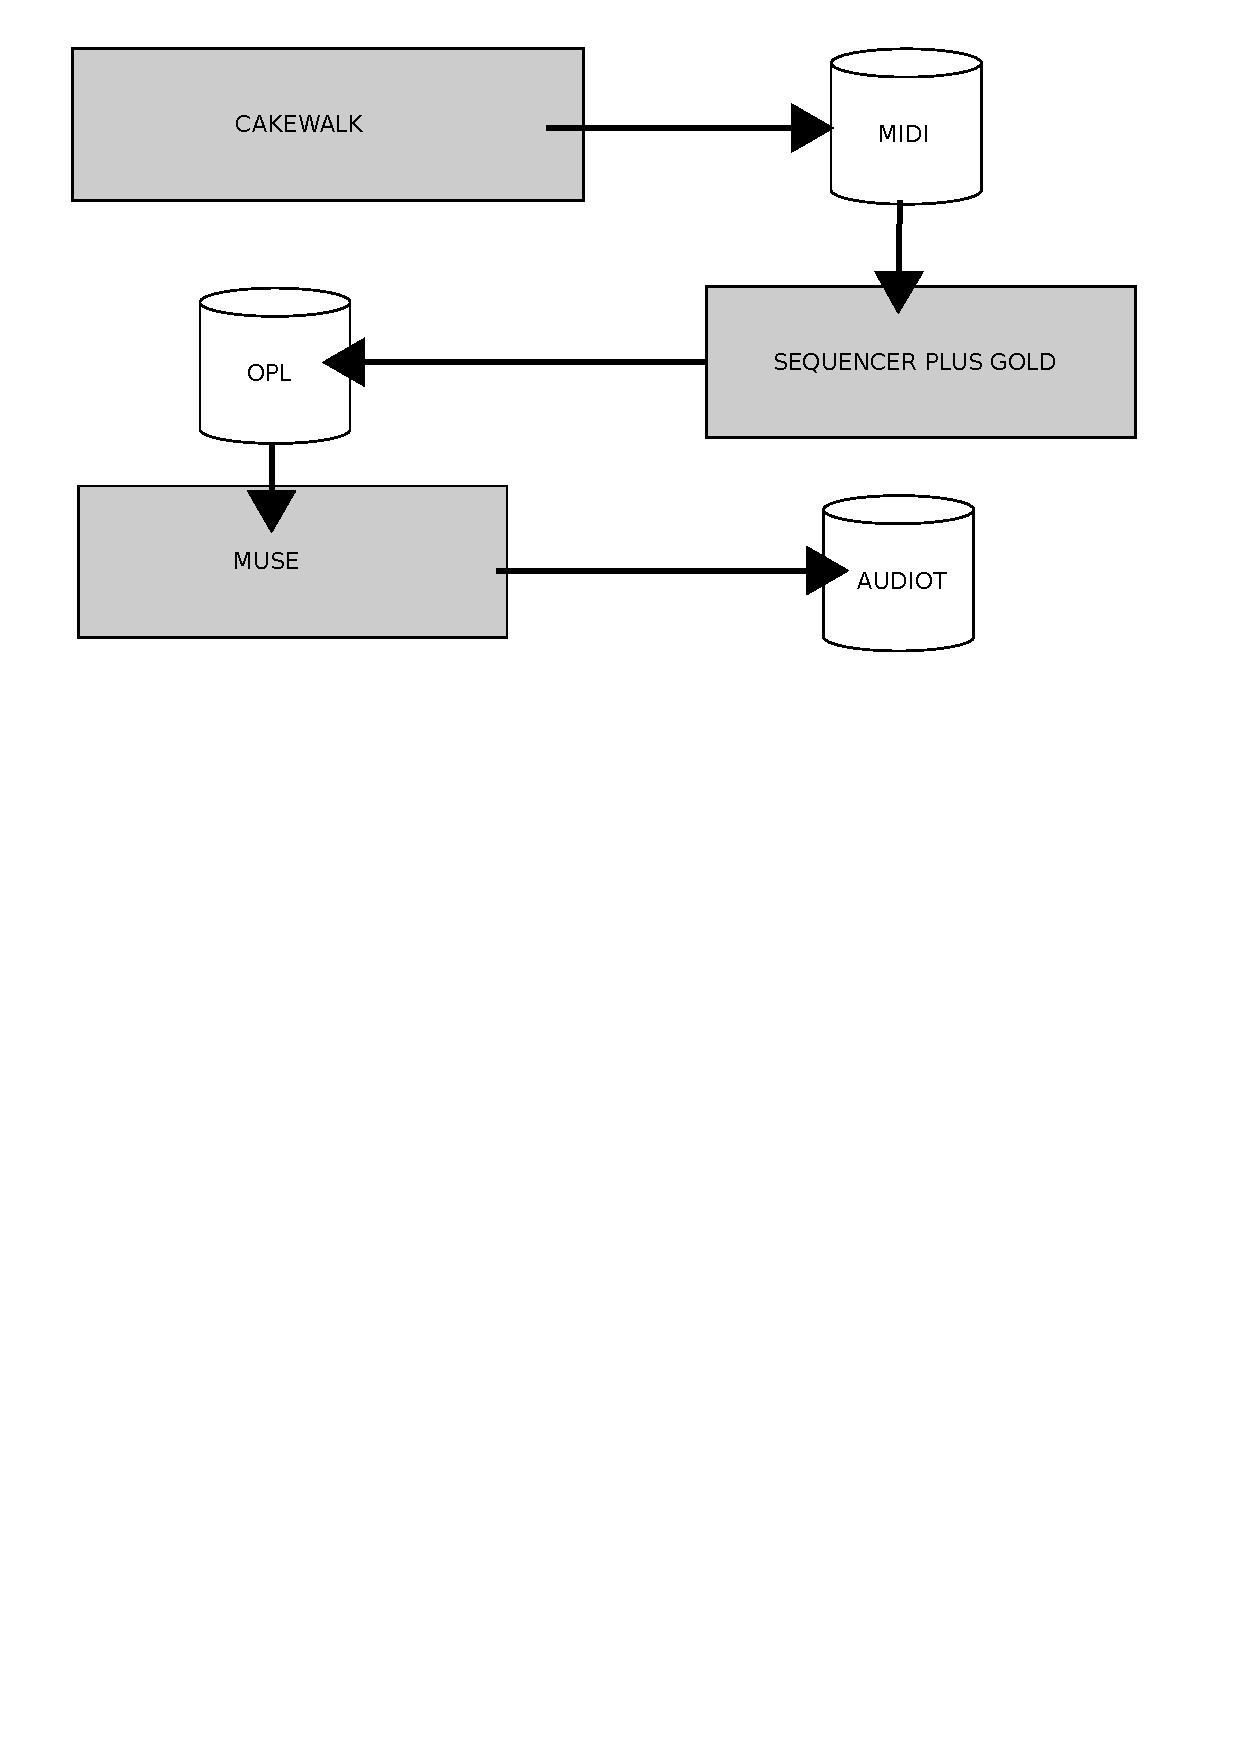
\includegraphics[width=\textwidth]{imgs/drawings/music_pipelione.pdf}
 \caption{Music pipeline as described by Bobby Prince.}
\end{figure}
The OPL format is also called IMF\footnote{Id software Music File}. Because it supports only the YM3812, it is tailored for the chip with zero abstraction layer. It consists of a stream of machine language commands with associated delays. The stream pilots the nine channels in the OPL2. A channel is able to simulate an instrument and play notes thanks to two oscillators, one playing the role of a modulator and the other the role of a carrier. There are many other ways to control a channel such as envelope, frequency or octave. The way a channel is programmed is described in detail in the "Software" chapter.
\begin{figure}[H]
\centering
 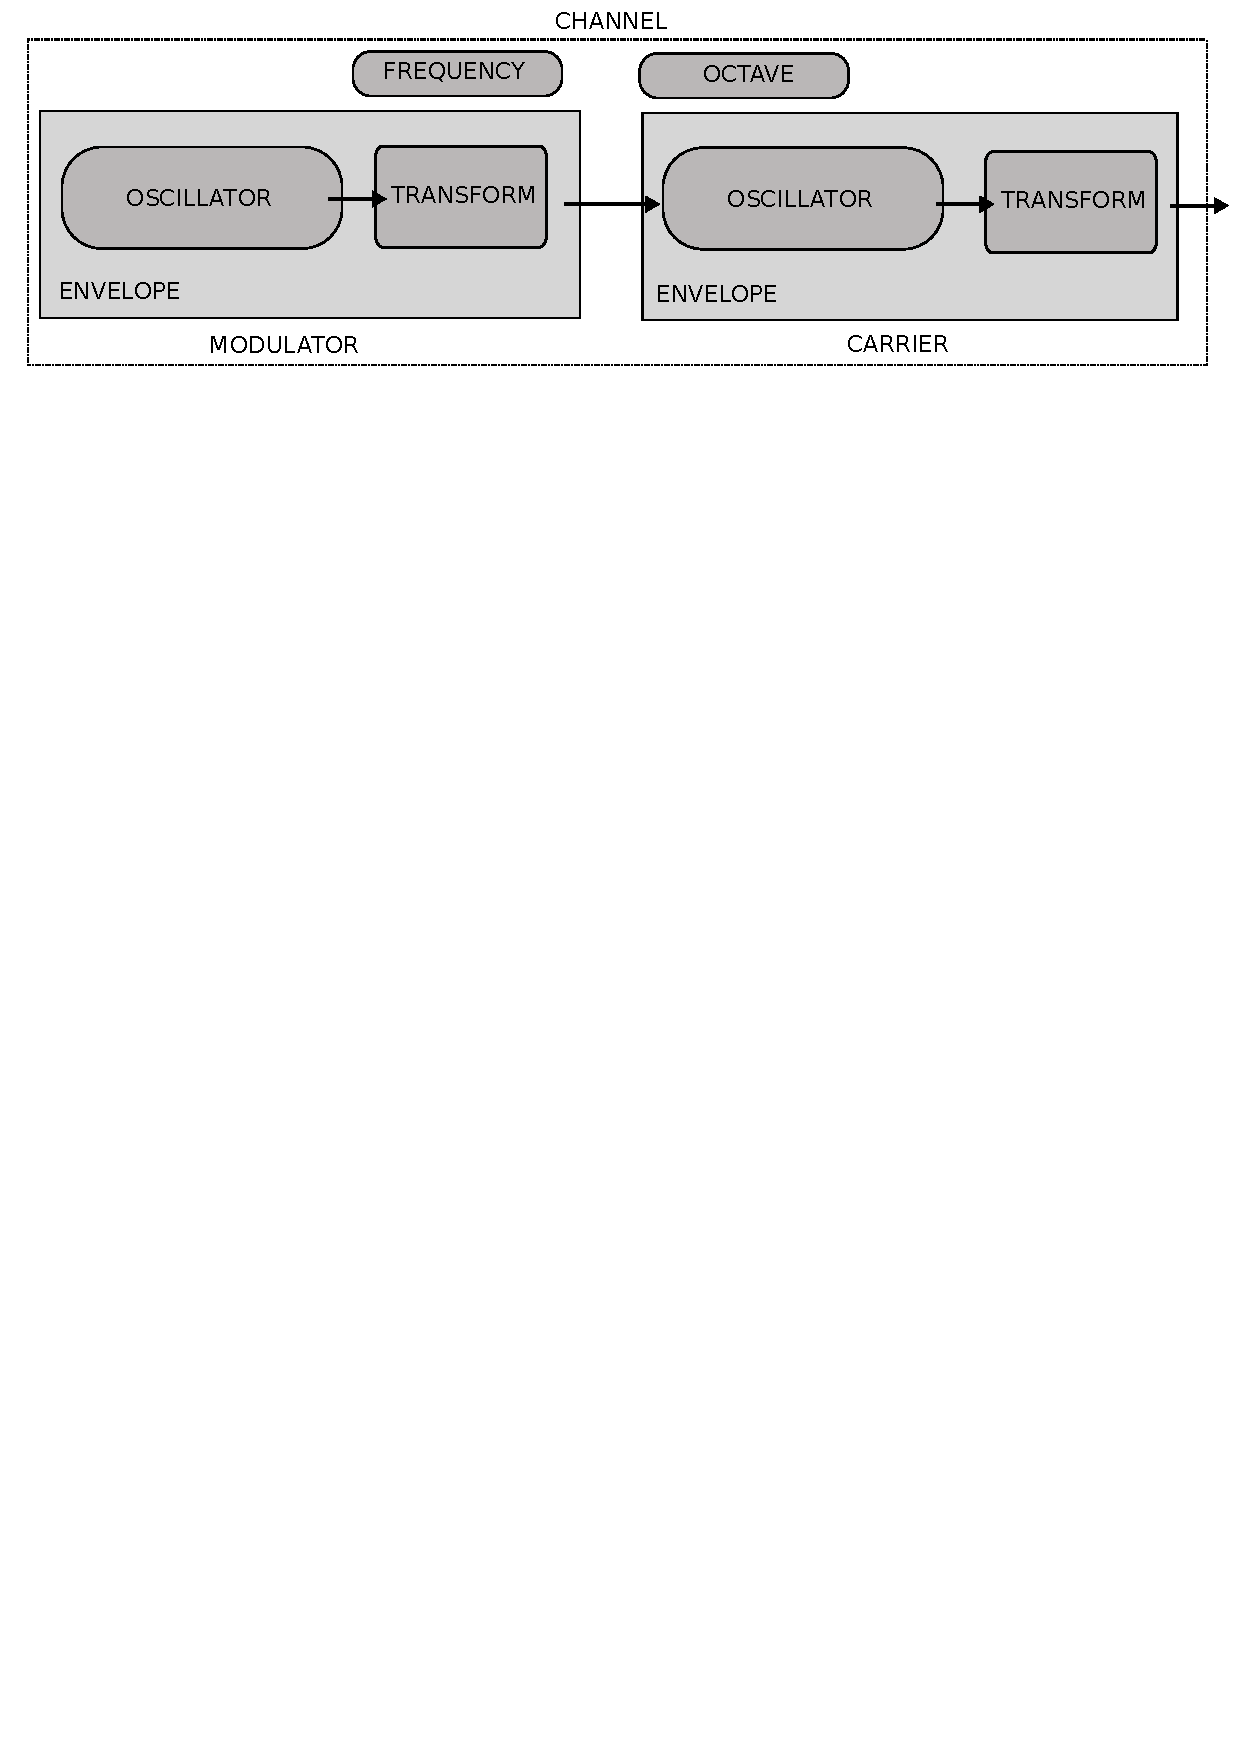
\includegraphics[width=\textwidth]{imgs/drawings/channel.pdf}
\end{figure}
\par
\bu{Trivia :}  The YM3812's unmistakable sonority is due to its pecular set of waveform transformer (they are right after the output of each oscillator in the drawing). Four waveforms are available on the OPL2.
\par
\begin{figure}[H]
\centering
 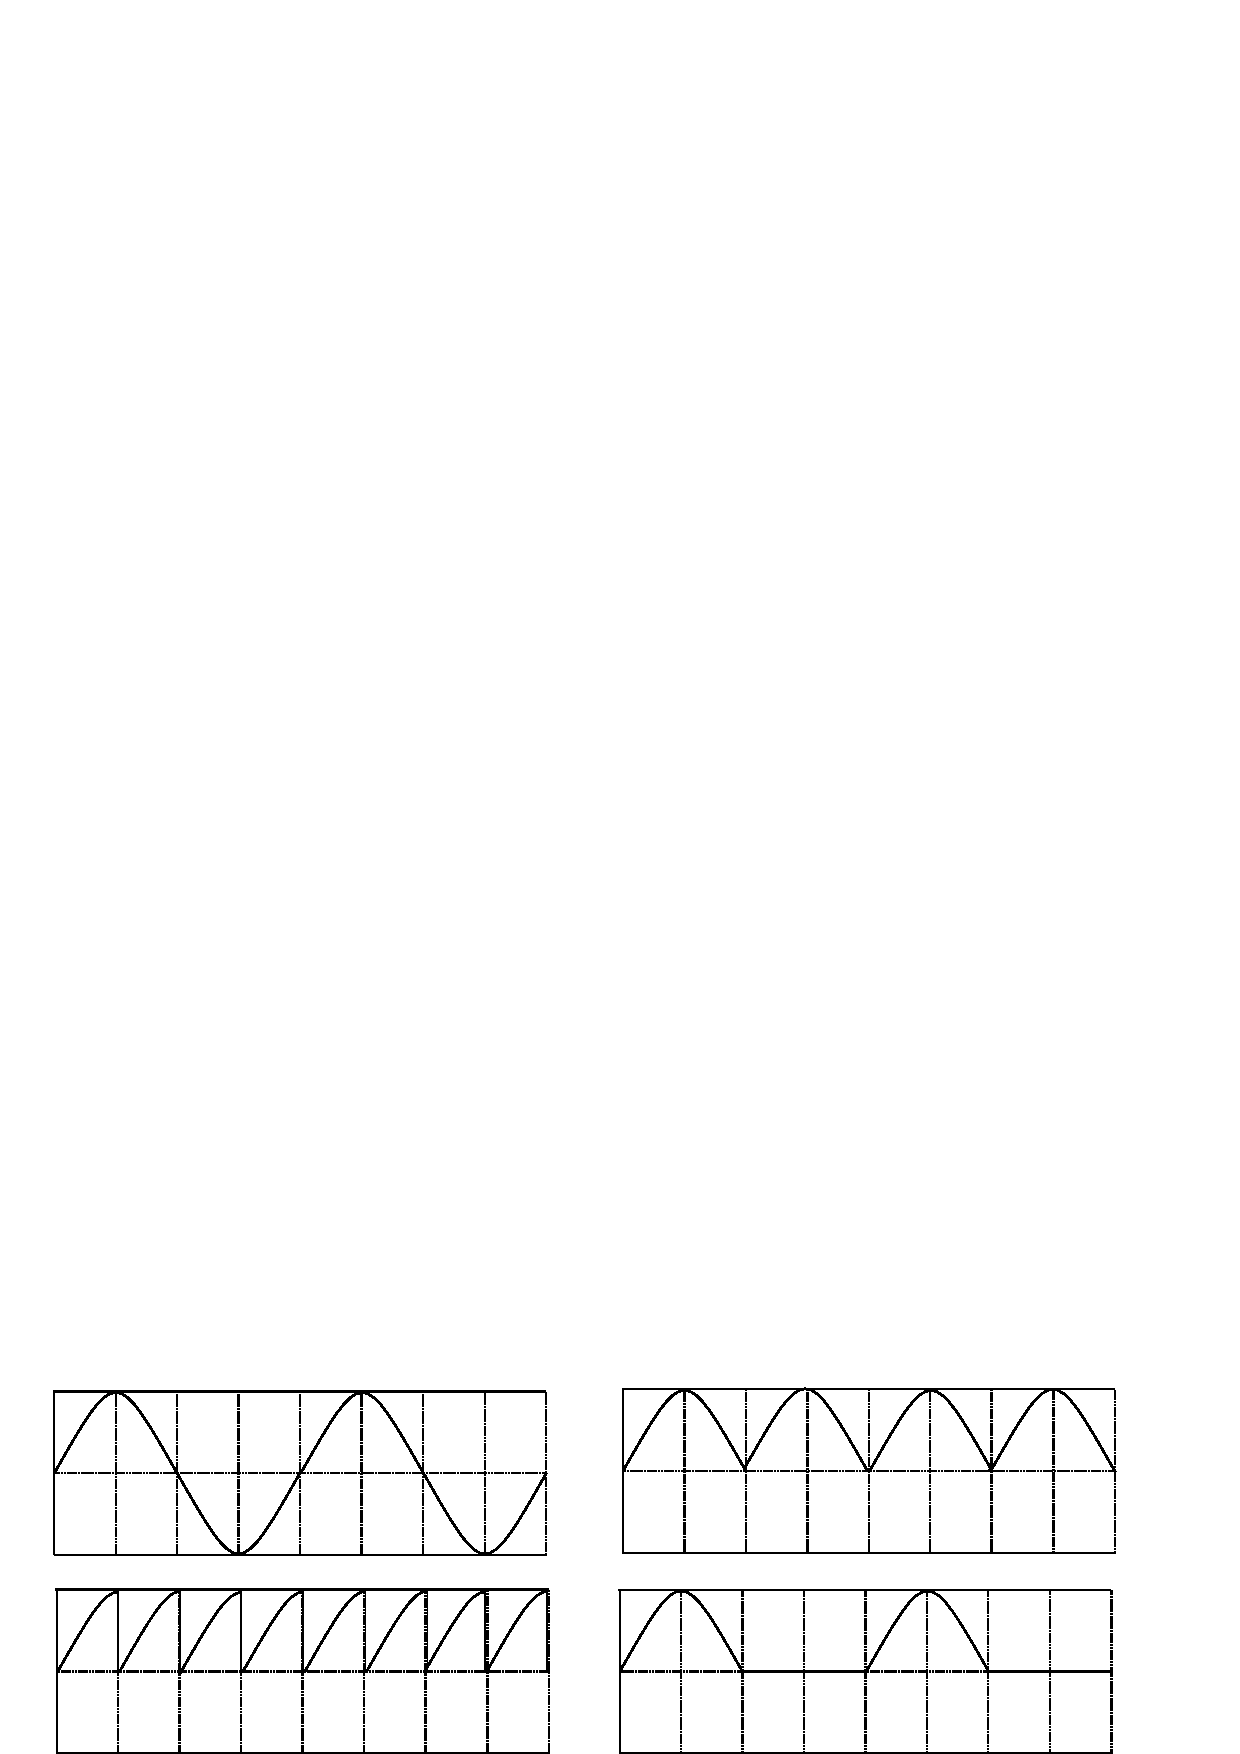
\includegraphics[width=\textwidth]{imgs/drawings/wave_transform.pdf}
\end{figure}


\bu{Trivia :} In Episode 3 the music playing features a hidden Morse coded message. "To Big Bad Wolf. De Little Red Riding Hood. Eliminate Hitler. Imperative. Complete mission within 24 hours. Out.". The end boss of this episode indeed is Hitler in a Mech suit (see hint drawing).




























\section{Distribution}
At 4am on May 5th, 1992 the first episode of the game was uploaded to Massachusetts via Software Creations BBS\footnote{Bulletin Board Systems where server allowing users to connect via a console and upload/download programs} server. Wolfenstein 3D was distributed as a shareware where only the game engine and the first episode of the game are given for free and encouraged to be copied and distributed to a maximum number of peoples. To receive the five other episodes each player had to send \$50 to id Software.\\
\par
\begin{figure}[H]
\centering
 \fullimage{shareware.png}
 \caption{Exiting the game describes how to get the full version.}
 \end{figure}

\end{document}
\par
In order to maximize income, it was therefore paramount to make the game easy to copy and redistribute. In 1991, Internet was still in its infancy and the best medium was the 3\nicefrac{1}{2}-inch floppy disk. Particular attention was given to the total size of the game so it would fit on one disk. All assets combined accounted for 1,204KiB but everything was compressed to 645KiB (a 3\nicefrac{1}{2}-inch floppy can store 720KB). The full six episodes fit on two disks. Spears of Destiny would fit on three disks.
The game shipped as follows:\\
\par
 \begin{figure}[H]
\centering
 \fullimage{result.png}
 \caption{All files distributed as shareware as they appear in DOS command prompt.}
  \end{figure}
  \par
 The files can be divided in five parts:
 \begin{itemize}
 \item WOLF3D.EXE: The Game engine.
 \item VSWAP.WL1: Contains all the assets (sprites, textures, digitized sound) needed during 3D action phases.
 \item Music files used during both 3D and 2D phases:
     \begin{itemize}
     \item AUDIOHED.WL1 : Index to payload in \cw{AUDIOT} file.
     \item AUDIOT.WL1: Uncompressed audio data. 
     \end{itemize}
\item Maps:
     \begin{itemize}
     \item MAPHEAD.WL1 : Index into \cw{GAMEMAPS} file.
      \item GAMEMAPS.WL1 : Compressed Map payloads.
      \end{itemize}
\item Pictures used during 2D menus phase:
    \begin{itemize} 
    \item VGAHEAD.WL1 : Index into \cw{VGAGRAPH} file.
    \item VGADICT.WL1 : Huffman-tree to decompress each the picture.
    \item VGAGRAPH.WL1 : Compressed pics lumped together.
     \end{itemize}
\end{itemize}
 \par

\textbf{\underline{Trivia :}} The file extension did have a meaning: 
\begin{itemize}
\item WL1: Shareware.
\item WL3: Early three-episode full version (never released).
\item WL6: Six-episode full version.
\item WJ1: Japanese shareware.
\item WJ6: Japanese full version.
\item SOD: Spear of Destiny.
\end{itemize}
 
\textbf{\underline{Trivia :}}The engine is very tiny and only uses 94KiB in total. But with 64KiB dedicated to the Signon screen (and 768B for the palette), the engine is in fact only 29KB.\\
\par
\begin{figure}[H]
\centering
\scaledimage{0.7}{disk.png}\\
\end{figure}
\par
Above, a 3\nicefrac{1}{2}-inch floppy widely used to share and redistribute the game. The upper left hole allows the disk reader to recognize if the disk is a low capacity (720 KiB) or a high capacity (1.44 MiB), The upper right hole features a sliding tab which when obstructing the hole forbids writting to the disk, making it read-only. Once inserted in the floppy disk reader, the metalic part slides to the right to expose the magnetic disk.
